\section{Computational Specifications and Training Times} \label{sec:com_train}

This section specifies the computational hardware used during the development of the model. Here, we detail the machines employed during training and testing and the time each part of this process consumes. Table \ref{tab:hardware} shows the GPU models used and the training times for each dataset configuration and part of the model. The RTX 3070 was available on a personal computer, while the Tesla T4 and RTX 4090 were run as servers. The availability of the computational resources in the workspace determined the usage of different machines. Besides the time spent on training, the model's performance does not depend on the GPU. The headers ``Central Square'' and ``Whole City'' should be interpreted as the ``Time to train - (in minutes, per epoch per source city) in this dataset configuration''.


%\begin{table}[]
%\begin{tabular}{llllll}
%\multicolumn{1}{c}{}          & \multicolumn{1}{c}{}    & \multicolumn{2}{c}{\textbf{Central Square}}       & \multicolumn{2}{c}{\textbf{Whole city}} \\ \hline
%\multicolumn{1}{c|}{GPU Model} & \multicolumn{1}{c|}{VRAM (GB)} & \multicolumn{1}{l|}{AE} & \multicolumn{1}{l|}{PRED} & \multicolumn{1}{l|}{AE} & PRED \\ \hline
%\multicolumn{1}{l|}{RTX 3070} & \multicolumn{1}{l|}{8}  & \multicolumn{1}{l|}{}   & \multicolumn{1}{l|}{}   & \multicolumn{1}{l|}{}         &         \\ \hline
%\multicolumn{1}{l|}{Tesla T4} & \multicolumn{1}{l|}{16} & \multicolumn{1}{l|}{60} & \multicolumn{1}{l|}{30} & \multicolumn{1}{l|}{}         &         \\ \hline
%\multicolumn{1}{l|}{RTX 4090} & \multicolumn{1}{l|}{24} & \multicolumn{1}{l|}{}   & \multicolumn{1}{l|}{}   & \multicolumn{1}{l|}{}         &         \\ \hline
%\end{tabular}
%\caption{Hardware specifications and training times}
%\label{tab:hardware}
%\end{table}

\begin{table}[!ht]
\begin{tabularx}{\textwidth}{ M | M | M | M | M | M }
\multicolumn{1}{X}{\textbf{GPU Model}}%
& \multicolumn{1}{X}{\textbf{VRAM (GB)}} 
& \multicolumn{2}{X}{\textbf{Central Square}}
& \multicolumn{2}{X}{\textbf{Whole City}} \\ \cline{3-6}
\multicolumn{1}{X}{}
& \multicolumn{1}{X}{}
& \multicolumn{1}{X}{\textbf{AE}}
& \multicolumn{1}{|X|}{\textbf{PRED}}
& \multicolumn{1}{|X|}{\textbf{AE}}
& \multicolumn{1}{X}{\textbf{PRED}} \\ \hline
RTX 3070 & 8 & 150 & 75 & & \\ \hline
Tesla T4 & 16 & 60 & 30 & & \\ \hline
RTX 4090 & 24 & & & & 
\end{tabularx}
\caption{Hardware specifications and training times}
\label{tab:hardware}
\end{table}

As observed in the Table, the training process is very time-consuming, even for powerful graphic cards. This is why, for the preliminary experiments, we chose to use only the Central Square of each city.

% autoencoder pre-training: 1 hour/epoch*N_cities
% autoencoder fine-tuning: 4 minutes/epoch
% predictor pre-training: 30 minutes/epoch*N_cities
% predictor fine-tuning: 2 minutes/epoch

% results in ~1h40/epoch*N_cities for training the model
% (collapsed channels, reduced city)
% one could expect the ``price'' to be then 1h40*10(size multiplier)*4(channels multiplier)= 60 hours/epoch*N_cities to train a full model
% training with only two epochs, one city: 120 hours = 5 days
% training with only two epochs, two cities: 240 hours = 10 days

\section{Autoencoder Experiments}

This Section will present the experiments on the variation of the autoencoder's parameters. Experiments \ref{ssec:exp1} to \ref{ssec:exp5} are related to the hyperparameter search for the autoencoder, while \ref{ssec:exp6} presents the impacts that parameter sharing as a domain adaptation technique.

Table \ref{tab:params_ae} shows the parameters used for most experiments in this Section. Note that when a different value is used for a determined experiment, this value would be stated on a similar table in the experiment explanation.

\begin{table}[!ht]
\begin{tabularx}{\textwidth}{ M | M }
\multicolumn{1}{X}{\textbf{Parameter}}%
& \multicolumn{1}{X}{\textbf{Value}} \\ \hline
Batch size                                  &  32                            \\ \hline
Number of cities                         & 2                            \\ \hline
Epochs                                       & 2                            \\ \hline
Chebyshev polynomial degree  & 2                            \\ \hline
Convolution dimension              & 16                           \\ \hline
Linear dimension                       & 8                            \\ \hline
Activation function                   & ReLU                      \\ \hline
Dropout rate                            & 0.5                         \\ \hline
Loss criterion                            & ZeroInflationLoss($w=100$)
\end{tabularx}
\caption{Fixed parameters for the autoencoder experiments}
\label{tab:params_ae}
\end{table}


\subsection{Experiment 1: Impact of the Chebyshev polynomial degree parameter on the autoencoder's performance} \label{ssec:exp1}


The Chebyshev polynomial degree is one of the parameters of the \texttt{GConvLSTM} cell used as the backbone of the autoencoder. It dictates the receptive field of the model, as it limits the number of neighbors that will be used to structure a computational graph during backpropagation. For instance, for a value of $K_{\text{cheb}}=1$, the computational graph will have a depth of 1, and only the nodes individually will be part of it. A $K_{\text{cheb}}=2$ implies that the computational graphs will contain not only the nodes themselves but the immediate neighbors of each node.

In this experiment, we evaluated the autoencoder's performance with varying values of \( K_{\text{cheb}} \), ranging from 1 to 6, while maintaining all other parameters as specified in Table \ref{tab:params_ae}. Figure \ref{fig:exp01boxplot} illustrates the distributions of both \gls{MAE} and \gls{MSE} for the corresponding \( K_{\text{cheb}} \) values. The boxplots reveal a discernible trend where both \gls{MAE} and \gls{MSE} metrics decrease as \( K_{\text{cheb}} \) increases from 1 up to 3, indicative of improved performance. The median of \gls{MAE} reaches its minimum at \( K_{\text{cheb}} = 3 \), suggesting this is the optimal Chebyshev polynomial degree for capturing the \gls{ST} features within the dataset, given the current parameter configuration. However, for \( K_{\text{cheb}} \) values greater than 3, there is an observable increase in variance and a slight rise in error metrics, which may signal a risk of overfitting. 

\begin{figure}[!ht]
\noindent\hspace{0.5mm}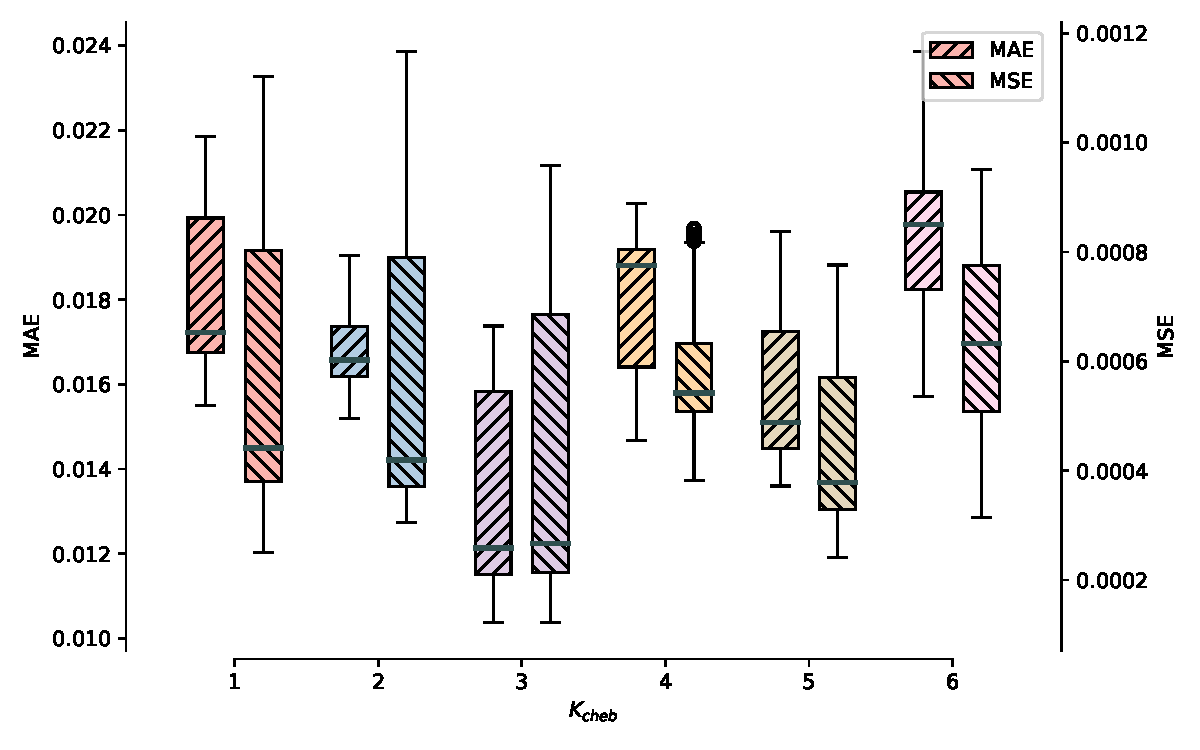
\includegraphics[width=0.9\textwidth]{./figures/exp01/boxplot.pdf}
\caption{\gls{MAE} and \gls{MSE} for the autoencoder with different values of $K_{\text{cheb}}$}
\label{fig:exp01boxplot}
\end{figure}


\subsection{Experiment 2: Impact of the number of source cities on the autoencoder's performance} \label{ssec:exp2}


\begin{table}[!ht]
\begin{tabularx}{\textwidth}{ M | M }
\multicolumn{1}{X}{\textbf{Parameter}}%
& \multicolumn{1}{X}{\textbf{Value}} \\ \hline
Batch size                                  & 8                            \\ \hline
\end{tabularx}
\caption{Specific parameters for Experiment 2}
\label{tab:exp02}
\end{table}

Experiment 2 deals with the impact of the number of cities on the autoencoder's performance. The number of cities indicates the data available to the model and the diversity and complexity presented. Four different values for the number of cities were considered: 1, 2, 4, and 8. The fixed parameters of the experiment are presented in Tables \ref{tab:params_ae} and \ref{tab:exp02}, and Figure \ref{fig:exp02boxplot} shows the results obtained.

For training over just one city $(N_{cities}=1)$, we observe a relatively high median value for both \gls{MAE} and \gls{MSE}, with a wide \gls{IQR}, suggesting that the model lacks generalization capabilities compared to the other models. Introducing another city to the model $(N_{cities}=2)$ seems to result in a slighter better median for the \gls{MSE}, but at the cost of outliers and a significantly higher median value for the \gls{MAE}. 

When training over four $(N_{cities}=4)$ and eight $(N_{cities}=8)$ cities, the model seem to behave similarly. It's noticeably better than the previous models when comparing the median values for both metrics, indicating better performance and generalization capabilities. There are outliers at $(N_{cities}=8)$, which may indicate a limit on how much diversity can be inputted into the model while trying to increase generalization capabilities.

The overall trend suggests that incorporating data from more cities enables the model to learn more generalizable features across different domains, reducing the model's bias toward specific cities' traffic patterns. It's worth noting that increasing the number of cities also increases the computational cost of training the model. Therefore, using the $N_{cities}$ values near 4 seems more optimal.

\begin{figure}[!ht]
\noindent\hspace{0.5mm}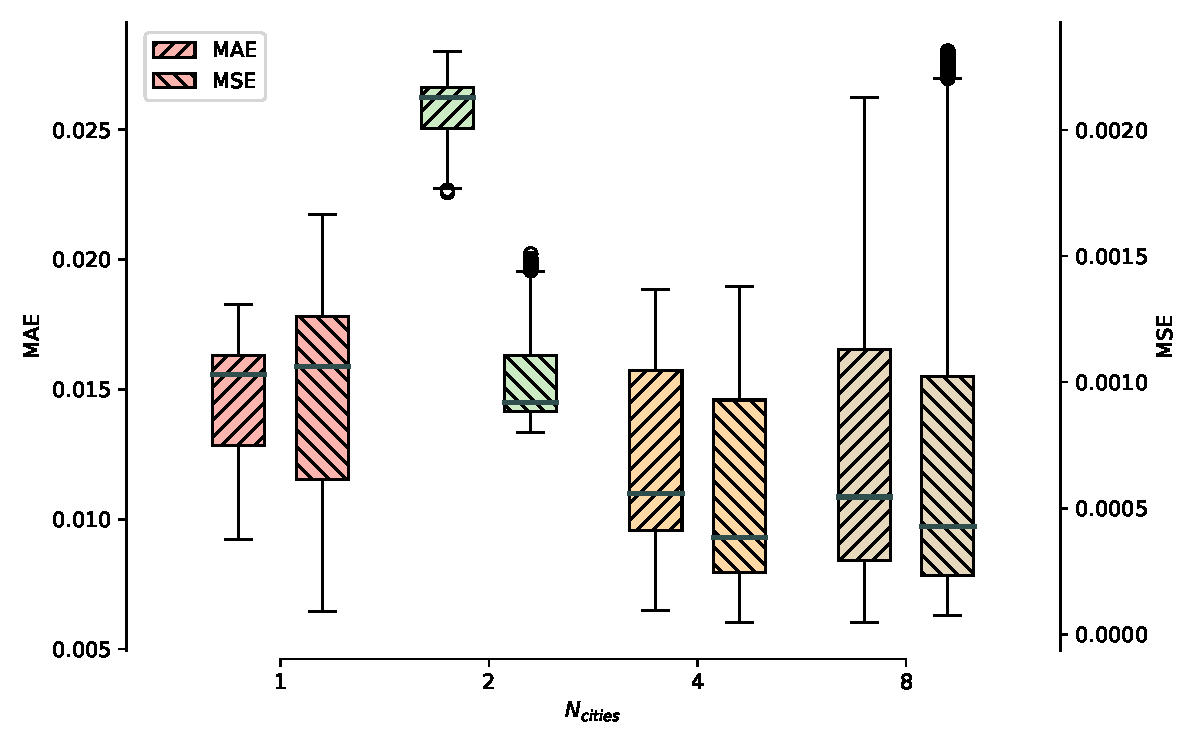
\includegraphics[width=0.9\textwidth]{./figures/exp02/boxplot.pdf}
\caption{\gls{MAE} and \gls{MSE} for the autoencoder with different number of cities}
\label{fig:exp02boxplot}
\end{figure}

\subsection{Experiment 3: Impact of the activation function on the autoencoder's performance} \label{ssec:exp3}


\begin{table}[!ht]
\begin{tabularx}{\textwidth}{ M | M }
\multicolumn{1}{X}{\textbf{Parameter}}%
& \multicolumn{1}{X}{\textbf{Value}} \\ \hline
Chebyshev polynomial degree  & 3                            \\ \hline
\end{tabularx}
\caption{Specific parameters for Experiment 3}
\label{tab:exp03}
\end{table}

The choice of activation function within neural network layers substantially impacts the model's ability to capture and represent complex patterns within the data. This experiment examines how the activation function selection influences the autoencoder's performance. Three standard activation functions were considered: ReLU, Sigmoid, and Tanh.

For this analysis, we trained separate autoencoder models using each activation function while keeping all other parameters constant, as specified in Tables \ref{tab:params_ae} and \ref{tab:exp03}. Figure \ref{fig:exp03boxplot} presents the distributions of \gls{MAE} and \gls{MSE} across the different activation functions.

The boxplots indicate that the model with the ReLU activation function exhibits a slightly higher median \gls{MAE} than the other functions but also has a broader \gls{IQR}, suggesting less consistent predictions across different instances. On the other hand, the model utilizing the Sigmoid function shows a tighter \gls{IQR} in \gls{MAE}, indicating less variability in its predictions. However, its median \gls{MAE} is higher. Interestingly, the Tanh function yields the lowest median \gls{MAE}, suggesting it may be the most effective at capturing the underlying \gls{ST} patterns for this dataset and model configuration.


\begin{figure}[!ht]
\noindent\hspace{0.5mm}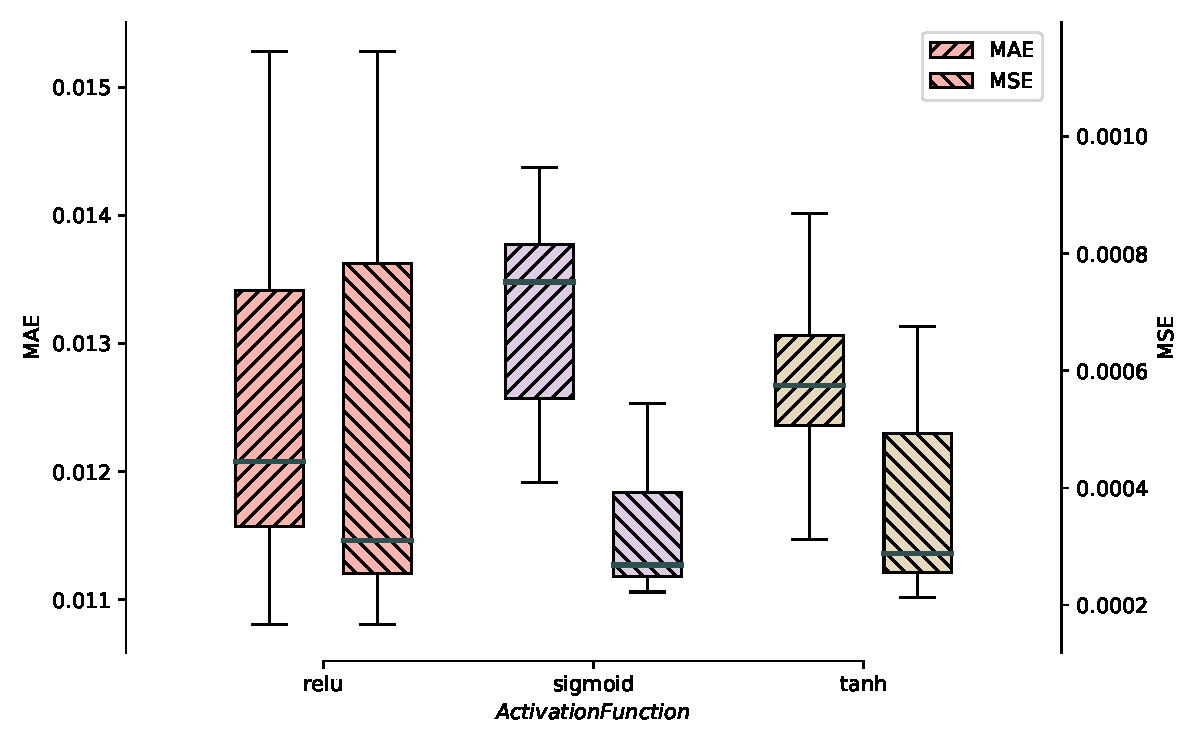
\includegraphics[width=0.9\textwidth]{./figures/exp03/boxplot.pdf}
\caption{\gls{MAE} and \gls{MSE} for the autoencoder with different activation functions.}
\label{fig:exp03boxplot}
\end{figure}


\subsection{Experiment 4: Impact of the criterion function on the autoencoder's performance} \label{ssec:exp4}


\begin{table}[!ht]
\begin{tabularx}{\textwidth}{ M | M }
\multicolumn{1}{X}{\textbf{Parameter}}%
& \multicolumn{1}{X}{\textbf{Value}} \\ \hline
Chebyshev polynomial degree  & 4                            \\ \hline
\end{tabularx}
\caption{Specific parameters for Experiment 4}
\label{tab:exp04}
\end{table}

Another interesting choice that can be made in the autoencoder training is the criterion function that yields the backpropagated loss. In this experiment, we analyze how different loss functions can influence the autoencoder's performance. All criteria used here were presented and explained in Section \ref{sec:loss_func}. All other parameters are exposed in Tables \ref{tab:params_ae} and \ref{tab:exp04}. The losses considered were:

\begin{itemize}
	\item \gls{MSE}
	\item \gls{WMSE} $(w=10)$
	\item \gls{WMSE} $(w=100)$
	\item \gls{MSLE}
	\item \gls{WMSLE} $(w=10)$
	\item \gls{WMSLE} $(w=100)$
	\item Log-Cosh Loss
	\item Focal Loss $(\alpha=0.25, \gamma=2)$
\end{itemize}

Figure \ref{fig:exp04boxplot} provides a comparative overview of the performance of these criteria on the autoencoder. From the plots, it is evident that both Focal Loss (with the input parameters) and Log-Cosh Loss are worse than their pairs, showing more considerable overall error (\gls{MAE} and \gls{MSE}) and \gls{IQR}, indicating that they are not fit for being used as criteria.

 The traditional \gls{MSE} provides a baseline for comparison, exhibiting a moderate spread in \gls{MAE} values. The \gls{MSLE} is designed to be less sensitive to significant errors by emphasizing the logarithmic difference between the predicted and actual values, which is evident in the lower median \gls{MAE} it achieves compared to \gls{MSE}.

A more nuanced approach is observed with both \gls{WMSE} and \gls{WMSLE}, where introducing a weight factor ($w$) aims to penalize errors differently based on their magnitude. Notably, for the \gls{WMSE}, as the weight increases from $w=1$ (\gls{MSE}) to $w=10$ to $w=100$, the spread and median of the \gls{MAE} decrease, suggesting a tighter grouping of errors around a lower central value. However, an increase in weight also introduces a higher variance in \gls{MSE}, as indicated by the presence of outliers, particularly for $w=100$. This implies that while \gls{WMSE} can potentially reduce the average error, it may also lead to more extreme errors in some instances. For the \gls{WMSLE} criterion, a similar result is observed, with the increase of $w$ being associated with a smaller \gls{IQR} but a higher median of the \gls{MAE}.

\begin{figure}[!ht]
\noindent\hspace{0.5mm}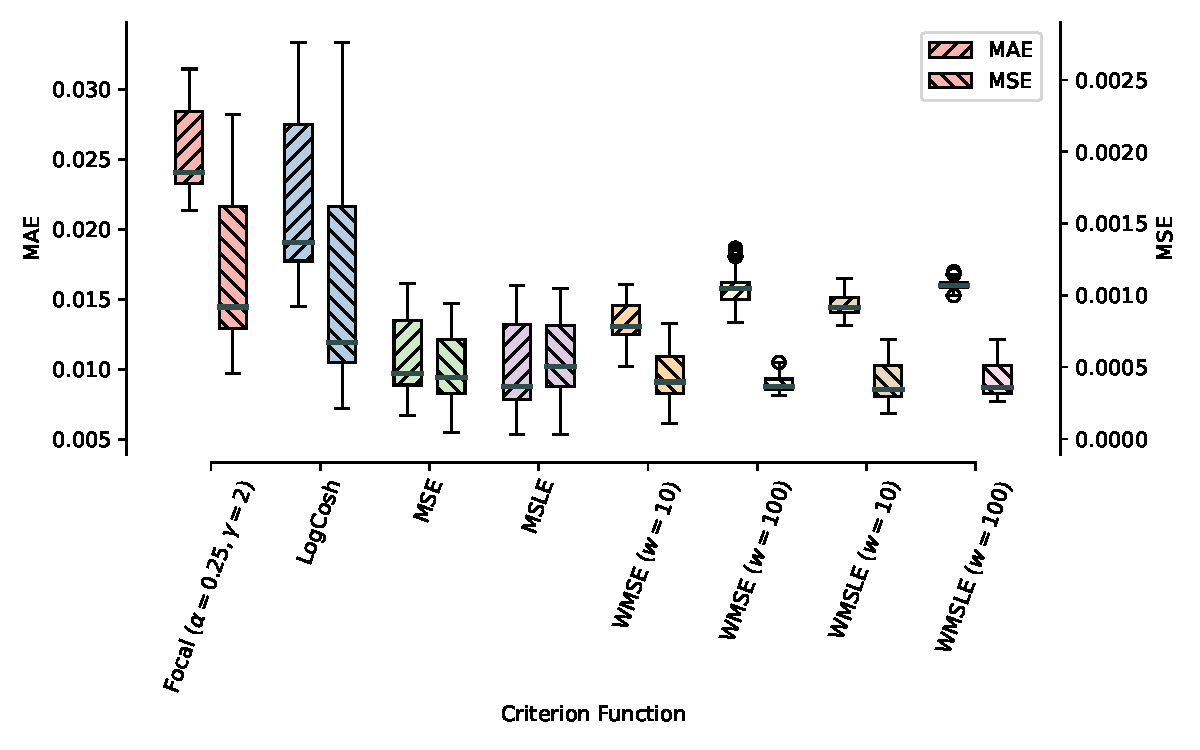
\includegraphics[width=0.9\textwidth]{./figures/exp04/boxplot.pdf}
\caption{\gls{MAE} and \gls{MSE} for the autoencoder with different criterion functions.}
\label{fig:exp04boxplot}
\end{figure}

\subsection{Experiment 5: Impact of the latent dimension's size the autoencoder's performance} \label{ssec:exp5}

\begin{table}[!ht]
\begin{tabularx}{\textwidth}{ M | M }
\multicolumn{1}{X}{\textbf{Parameter}}%
& \multicolumn{1}{X}{\textbf{Value}} \\ \hline
Chebyshev polynomial degree  & 4                            \\ \hline
Activation function                   & Tanh                      \\ \hline
\end{tabularx}
\caption{Specific parameters for Experiment 5}
\label{tab:exp05}
\end{table}

Experiment 5 focuses on the impact of inner (or latent) layer dimensions on the autoencoder's performance. For this purpose, several pairs of convolutional and linear dimensions were tested and are exposed in Tables \ref{tab:params_ae} and \ref{tab:exp05b}. Furthermore, Table \ref{tab:exp05} shows the fixed parameters for the experiment.

\begin{table}[!ht]
\begin{tabularx}{\textwidth}{ M | M }
\multicolumn{1}{X}{\textbf{Convolutional Dimension}}%
& \multicolumn{1}{X}{\textbf{Linear Dimension}} \\ \hline
8    & 2     \\ \hline
8    & 4    \\ \hline
8    & 8    \\ \hline
16  & 4    \\ \hline
16  & 8    \\ \hline
16  & 16  \\ \hline
32  & 8    \\ \hline
32  & 16
\end{tabularx}
\caption{Tested pairs of convolutional and linear dimensions.}
\label{tab:exp05b}
\end{table}

Analyzing Figure \ref{fig:exp05boxplot}, it's possible to note that the convolutional dimension is the most critical parameter between the two. Models with smaller convolutional dimensions ($\texttt{conv\_dim}=8$) tend to have higher \gls{MAE} and \gls{MSE} values, indicating a lower performance. This suggests that these models may not have enough complexity to capture the data's relevant \gls{ST} features.

Going up to $\texttt{conv\_dim}=16$, we can observe a significant reduction in both metrics. This points to a better extraction feature, enabling the autoencoder to capture more of the data's complexity. Finally, with $\texttt{conv\_dim}=32$, we note an increase of the median and extremes of the error, but a smaller \gls{IQR}, suggesting that we've reached a point where overfitting starts to take effect on the model.

Considering the values of the linear dimensions now, there's no clear trend that we can extract from the results, as an increase in it for low values of convolutional dimension led to more significant errors, but for other values, it made no difference. It's important to note that increasing convolutional and linear dimensions implies higher model complexity and, thus, higher computational cost for training it. For this reason, settling for pairs like $(16, 4)$ or $(16, 8)$ is the best option for balancing performance with cost.

\begin{figure}[!ht]
\noindent\hspace{0.5mm}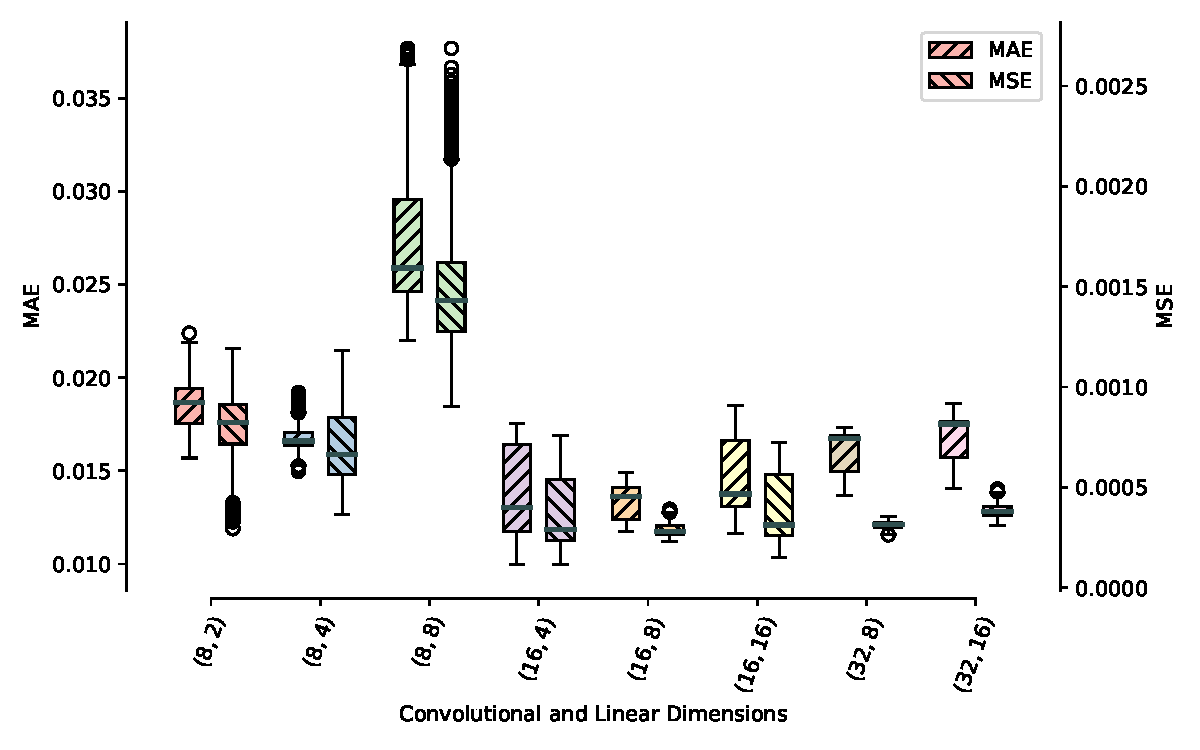
\includegraphics[width=0.9\textwidth]{./figures/exp05/boxplot.pdf}
\caption{\gls{MAE} and \gls{MSE} for the autoencoder with different pairs of latent dimension values.}
\label{fig:exp05boxplot}
\end{figure}

\subsection{Experiment 6: Pretraining as a domain adaptation technique for the autoencoder} \label{ssec:exp6}

\begin{table}[!ht]
\begin{tabularx}{\textwidth}{ M | M }
\multicolumn{1}{X}{\textbf{Parameter}}%
& \multicolumn{1}{X}{\textbf{Value}} \\ \hline
Batch size                                  & 16                         \\ \hline
Number of cities                        &  1                            \\ \hline
Epochs                                       & 4                            \\ \hline
Chebyshev polynomial degree  & 4                            \\ \hline
Activation function                   & TanH                      \\ \hline
\end{tabularx}
\caption{Specific parameters for Experiment 6}
\label{tab:exp06}
\end{table}

Experiment 6 is the first attempt to apply a fine-tuning technique to transfer knowledge from one model to another. It consisted of training the model across three different setups: using solely the target city data (``Target Only''), pretraining with data from one source city followed by finetuning on the target city data (``Pretrained w/ 1 Source''), and pretraining with data from two source cities before finetuning on the target city data (``Pretrained w/ 2 Sources''). The results, illustrated in Figure \ref{fig:exp06boxplot}, underscore the benefits of transfer learning through pretraining.

The ``Target Only'' model shows the higher median and \gls{IQR} for both \gls{MAE} and \gls{MSE} when compared to the pre-trained ones. Conversely, both pre-trained setups significantly reduce both error metrics' median and \gls{IQR}. This suggests that the pre-training is an effective method for domain adaptation, as the model gets significantly better at generalizing and accurately predicting the \gls{ST} patterns. Furthermore, the image also indicates that having more cities can enhance this technique, as the diversity of data presented in the model increases its generalization capacity, making it more accurate.

\begin{figure}[!ht]
\noindent\hspace{0.5mm}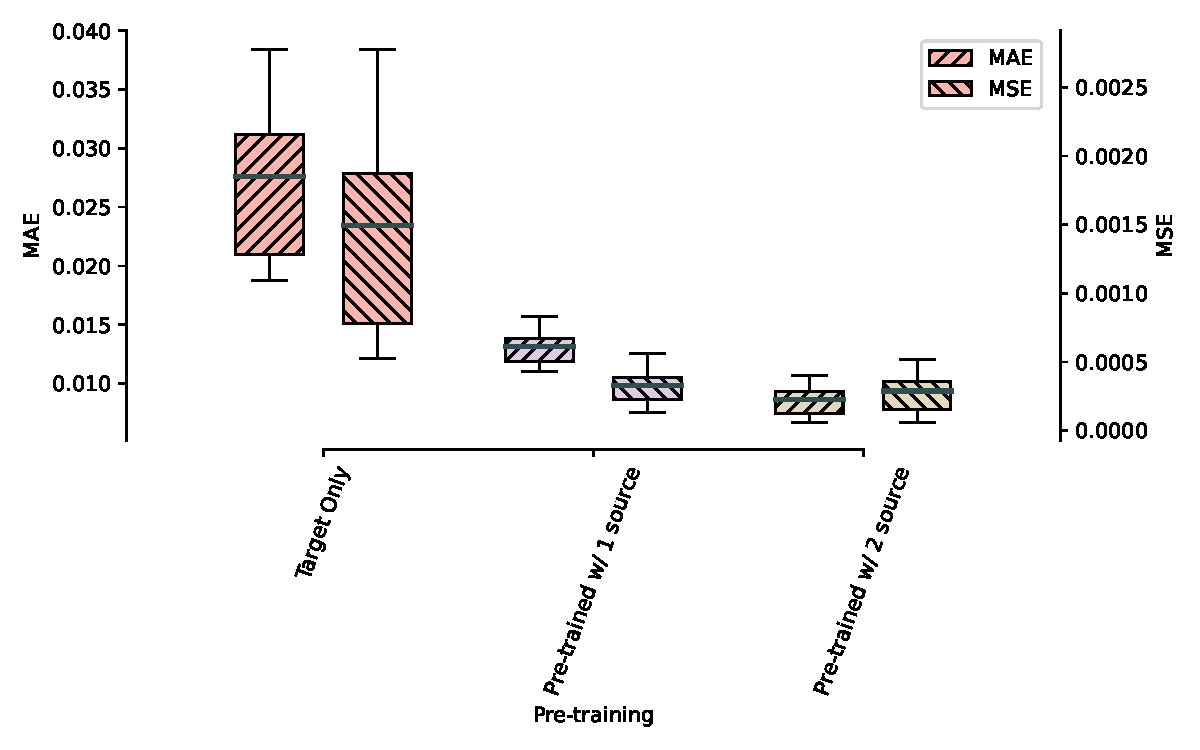
\includegraphics[width=0.9\textwidth]{./figures/exp06/boxplot.pdf}
\caption{\gls{MAE} and \gls{MSE} for the autoencoders using different pre-training strategies.}
\label{fig:exp06boxplot}
\end{figure}


\section{Predictor Experiments}

Given then an autoencoder capable of effectively extracting the relevant \gls{ST} features, it's necessary now to define good hyperparameters for the predictor part of the model. Experiments .... investigate the optimization of the model by parameter variation, while Experiments ... deal with the knowledge transfer part.

Similarly to how we organized the previous Section, Table \ref{tab:params_pred} shows the fixed parameters for all predictor experiments. If a parameter from this table is to be changed, it will be clearly stated on the particular experiment's specific parameters table.

\begin{table}[!ht]
\begin{tabularx}{\textwidth}{ M | M | M }
\multicolumn{1}{X}{\textbf{Module}}
& \multicolumn{1}{X}{\textbf{Parameter}}%
& \multicolumn{1}{X}{\textbf{Value}} \\ \hline
both & Batch size                                  & 64                          \\ \hline
both & Epochs                                       &  2                           \\ \hline
both & Number of source cities             & 1                            \\ \hline
both & Weeks of target data                             & 2            \\ \hline
\gls{AE} & Chebyshev polynomial degree  & 3                            \\ \hline
\gls{AE} & Convolution dimension              & 16                          \\ \hline
\gls{AE} & Autoencoder Linear dimension  & 8                            \\ \hline
\gls{AE} & Activation function                   & TanH                      \\ \hline
\gls{AE} &  Dropout rate                            & 0.5                         \\ \hline
\gls{AE} & Loss criterion                            & \gls{MSE}              \\ \hline
\gls{AE} & $\lambda$ regularization           & 0.1              \\ \hline
\gls{PRED} & Activation function              & ReLU                      \\ \hline
\gls{PRED} & Loss criterion                       & \gls{MSE}              \\ \hline
\gls{PRED} & Top-K Pooling                       & 1750            \\ \hline
\gls{PRED} & Linear Dimension                  & 32              
\end{tabularx}
\caption{Fixed parameters for Predictor experiments}
\label{tab:params_pred}
\end{table}


\todo[inline]{complete this introduction}


\subsection{Experiment 7: Impact of the lambda regularization on the predictor} \label{ssec:exp7}


As we complete the development of the autoencoder, it's essential to address one of the main challenges of the proposed model: to generalize the knowledge obtained on the source domain to the new, different target domain. As presented in the Methodology section, we aim to learn how to extract domain-invariant features, which hold the key to a model's ability to perform well across varied domains without succumbing to domain-specific biases.

In this context, Experiment 7 was designed to investigate the impact of balancing the reconstruction loss of the autoencoder with the domain discriminator loss, modulated by a regularization parameter $\lambda$. This parameter regulates the trade-off between the fidelity of the reconstruction and the degree of domain invariance imposed by the \gls{DD}. Since we're introducing a regularization technique in the model's training, we expect that the individual performance of the autoencoder must pay for this enhanced performance on the generalization of the features, as we try to ``fool'' it during training.

The values of $\lambda$ tested range from $0$ to $1$, including $0.001, 0.005, 0.01, 0.1, 0.5,$ and $1$. A value of $0$ means no regularization from the domain discriminator and, therefore, no adversarial training, while a value of $1$ means that reconstruction and domain discriminator losses have the same weight when composing the total loss.

Figure \ref{fig:exp07boxplot} exposes the results obtained from training these models. The plot suggests that including the domain discriminator loss positively impacts the model's prediction ability as the performance for $\lambda=0$ is inferior to that for $\lambda \neq 0$. In particular, we can observe that for the \gls{MAE} boxes, there's an apparent decrease in both median and max values when going from $\lambda=0$ to $\lambda=0.001$ and then from $\lambda=0.001$ to $\lambda=0.005$, from which point it's hard to observe significant changes on the performances. However, one can verify that the number of outliers on the maximum size of the boxes seems to increase.

One possible explanation for the lack of changes observed from a certain point onwards is that as we reach a point of stabilization during training, the reconstruction loss starts to reach low values (in the order of $10^{-4}$). At the same time, we maintain the domain discriminator loss oscillating around 0.6 (the ideal expected value for it is $\ln{(2)}\simeq 0.693$, which occurs when the domain discriminator can't identify the domain due to the features being completely domain-agnostic). This means that the domain discriminator loss, supposed constant, will dominate the total loss almost constantly, and, for a determined threshold, there's no difference between $\lambda=0.5$ and $\lambda=1$ as they both result in a seemingly significant loss for the optimizer.

\begin{figure}[!ht]
\noindent\hspace{0.5mm}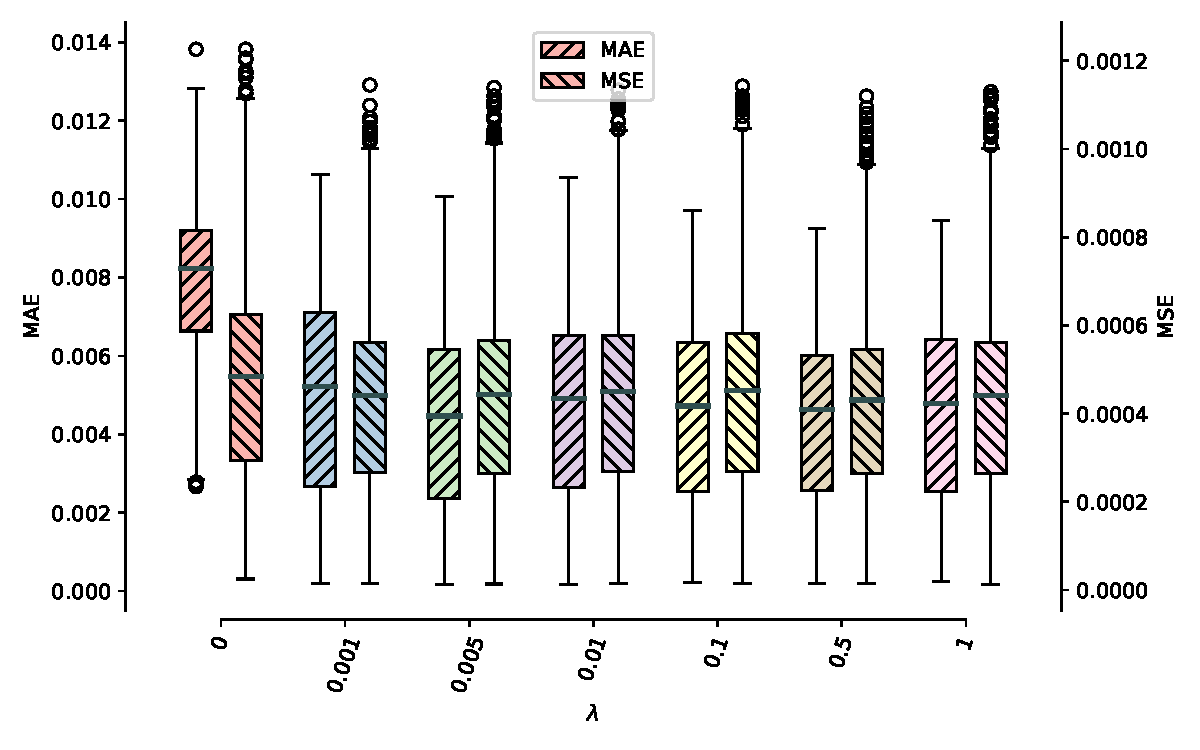
\includegraphics[width=0.9\textwidth]{./figures/exp07/boxplot.pdf}
\caption{\gls{MAE} and \gls{MSE} on the prediction using different values of $\lambda$.}
\label{fig:exp07boxplot}
\end{figure}

\subsection{Experiment 8: Impact of the linear layer dimension on the predictor} \label{ssec:exp8}

\begin{table}[!ht]
\begin{tabularx}{\textwidth}{ M | M | M }
\multicolumn{1}{X}{\textbf{Module}}
& \multicolumn{1}{X}{\textbf{Parameter}}%
& \multicolumn{1}{X}{\textbf{Value}} \\ \hline
\gls{PRED} & Activation function              & ReLU                      \\ \hline
\gls{PRED} & Loss criterion                       & \gls{MSE}              \\ \hline
\gls{PRED} & Top-K Pooling                       & 1750          
\end{tabularx}
\caption{Specific parameters for Experiment 8}
\label{tab:exp08}
\end{table}

Experiment 8 was projected to better understand the impact of the linear layer dimension, the output size of the \gls{A3T-GCN} layer, on the model's performance. The experiment assessed four sizes for the linear dimension: 8, 16, 32, and 64. Figure \ref{fig:exp08boxplot} shows the \gls{MAE} and \gls{MSE} distribution for the different compositions. With the increase in the size of the output of the convolutional block, the median of both metrics also increases, suggesting potential overfitting or a decrease in the model's ability to generalize.

\begin{figure}[!ht]
\noindent\hspace{0.5mm}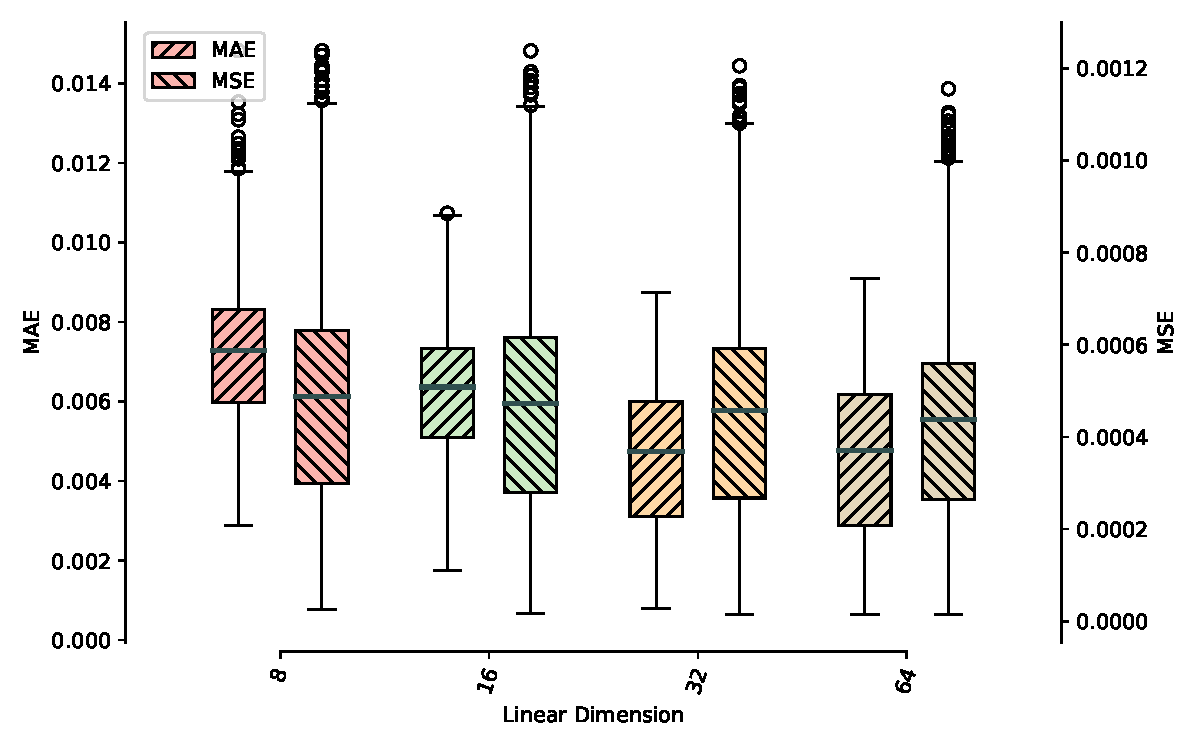
\includegraphics[width=0.9\textwidth]{./figures/exp08/boxplot.pdf}
\caption{\gls{MAE} and \gls{MSE} on the prediction using different domain adaptation techniques.}
\label{fig:exp08boxplot}
\end{figure}

\subsection{Experiment 9: impact of the number of epochs on the predictor}

In machine learning terms, an epoch represents a complete cycle through the data, providing the model with repeated exposure to the training examples and allowing it to incrementally adjust its parameters. Changing the number of epochs to be used impacts the model's performance directly, as an epoch count that is too low may lead to underfitting. At the same time, too many epochs can cause overfitting. This investigation is critical for understanding the temporal dynamics of model convergence and identifying the most resource-efficient training regimen that maintains or enhances model efficacy.

For this experiment, we tested the model proposed using five different values of the number of epochs, ranging from 1 to 5, to be used on the autoencoder and predictor training. Figure \ref{fig:exp09boxplot} contains the results obtained. There's a clear trend of improvement in the model's performance as we increase the number of training epochs. We can observe a considerable gap on both \gls{MAE} and \gls{MSE} from one to two epochs. Still, the rate of improvement appears to diminish after that, as the median for the remaining boxes seems to share similar medians and \gls{IQR}. Nonetheless, we can observe that the maximum error (for both metrics) continues to decrease with the increase of epochs. This indicates that the model is becoming more robust to outliers and noise in the data.

As we reach three training epochs, we've got a plateau regarding median error for the metrics, suggesting that the model may be approaching its learning capacity given the provided data. As we're dealing with a relatively large training dataset (in both numbers of data points and information/nodes per data point), it's plausible to consider that with only three epochs, the model has effectively learned how to capture the underlying patterns in the data. Since, as discussed in Section \ref{sec:com_train}, an epoch of training with one source city takes approximately two hours, given the computational resources available, we can consider that the modest number of three epochs is sufficient for the model to learn. We can allocate the processing power into other areas of the model, such as supporting more source cities.

\begin{figure}[!ht]
\noindent\hspace{0.5mm}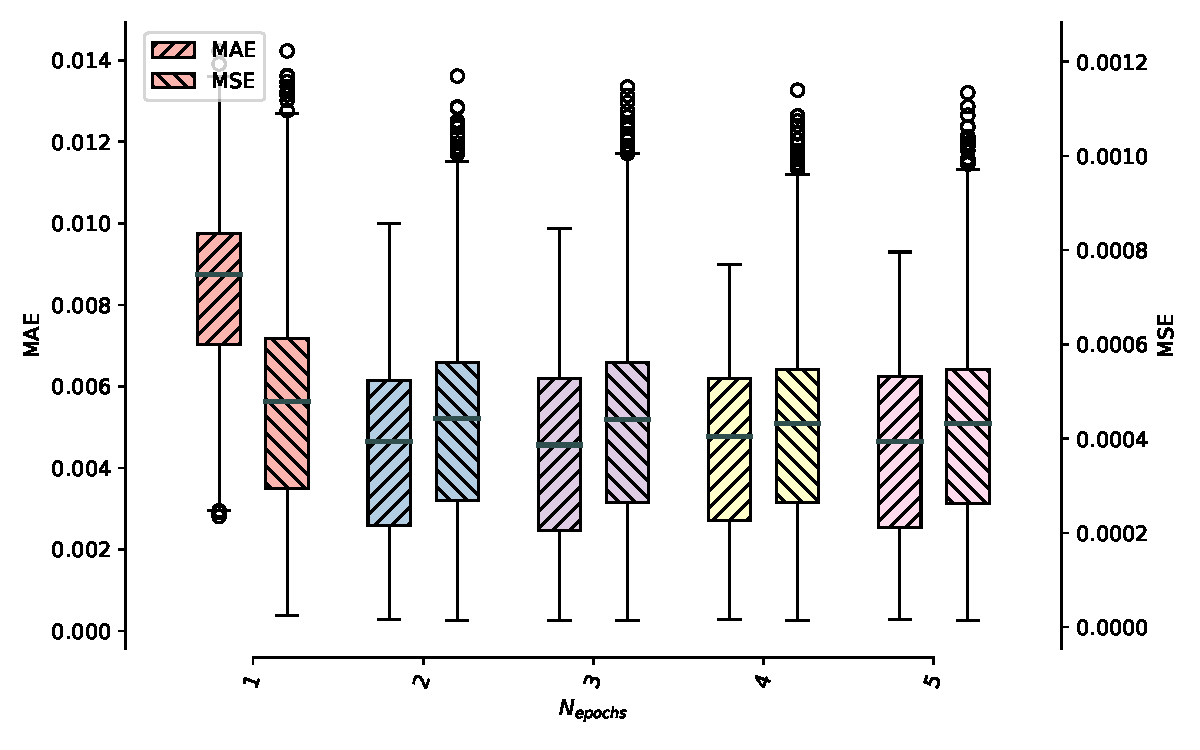
\includegraphics[width=0.9\textwidth]{./figures/exp09/boxplot.pdf}
\caption{\gls{MAE} and \gls{MSE} on the prediction using different number of epochs.}
\label{fig:exp09boxplot}
\end{figure}



\subsection{Experiment 10: Impact of the scarcity of the target dataset}

As the volume of available target data is one of the main grounds on which the development of transfer learning models is based, we find it interesting to experiment with how the availability of this kind of data impacts the overall performance of the model. By incrementally increasing the quantity of target data from 1 to 4 weeks, we aim to uncover how the breadth of target domain exposure affects the model's capacity to learn and generalize. Also, for many decision-makers, for which such models must yield important information that will govern their decisions, the availability of such data has a monetary price. By examining the model's performance with 1, 2, 3, and 4 weeks of target data, we can evaluate the prediction performance one can obtain for that price.



\section{Full Model Experiments}

Building upon the insights obtained from the previous experiments, we now assess the entire model, experimenting with the complete model in its best possible form. Also, to test the model in its best extension, for this Section, we use the entire city's data, not only the central square we've been using until now to save computation resources (as discussed in Section \ref{sec:data_analysis}).

Furthermore, for this section, the trained models will be tested against two baselines: \gls{ARIMA} and \gls{HA}, standard baselines in traffic prediction. All baselines and models are evaluated by three metrics: \gls{MAE}, \gls{MAPE}, and \gls{RMSE}.
